% siminos/CLE/introCLE.tex
% $Author$ $Date$

\subsection{\label{s:introCLE} An example: \CLe}
% introducing CLe
% from siminos/thesis/lasersSym.tex and
% ChaosBook chapter continuous.tex {Relativity for cyclists} 18 Jan 2010

Consider a complex generalization of Lorenz equations,
\bea
 \dot{x} &=& -\sigma x+ \sigma y \,,\qquad
 \dot{y} \,=\, (\rLor-z)x-a y \continue
 \dot{z} &=& (x y^*+x^*y)/2 -b z\,,
 \label{eq:CLe}
\eea
where $x,y$ are complex variables, $z$ is real, while the
parameters $\sigma,\,b$ are real and $\rLor=\RerCLor+i
\ImrCLor$, $a=1-i e$ are complex. Recast in real variables,
this is a set of five coupled ODEs
\bea
	\dot{x}_1 &=& -\sigma x_1 + \sigma y_1\continue
	\dot{x}_2 &=& -\sigma x_2 + \sigma y_2\continue
	\dot{y}_1 &=& (\RerCLor-z) x_1 - \ImrCLor x_2 -y_1-e y_2 \continue
	\dot{y}_2 &=& \ImrCLor x_1 + (\RerCLor-z) x_2 + e y_1- y_2\continue
	\dot{z} \; &=& -b z + x_1 y_1 + x_2 y_2
    \,.
\label{eq:CLeR}
\eea
In all numerical examples that follow, the parameters will be
set to $\RerCLor=28,\, \ImrCLor=0,\, b=8/3,\, \sigma=10,\, e=
1/10$, unless explicitly stated otherwise. Why worry about
continuous symmetries? This simple, 5-dimensional example
suffices to illustrate the effect a continuous symmetry has
on dynamics. \refFig{fig:CLE} offers a visualization of
typical long-time dynamics of the \cLf. A generic trajectory
slowly `drifts' along the direction of continuous symmetry
while tracing a Lorenz-butterfly like attractor. It is a
mess.
    \ES{Split \reffig{fig:CLE} into: Fig1: reqb, generic
    trajectory, rpo. Fig2: reqb, unstable manifolds}
    \PC{I would prefer to have a plot of long-time trajectory
        without exact solutions superimposed, as in ChaosBook
    refFig\,\{fig:CLEx1x2z\}.
    }
%
%%%%%%%%%%%%%%%%%%%%%%%%%%%%%%%%%%%%%%%%%%%%%%%%%%%%%%%%%%%%
\begin{figure}[ht]
\begin{center}
  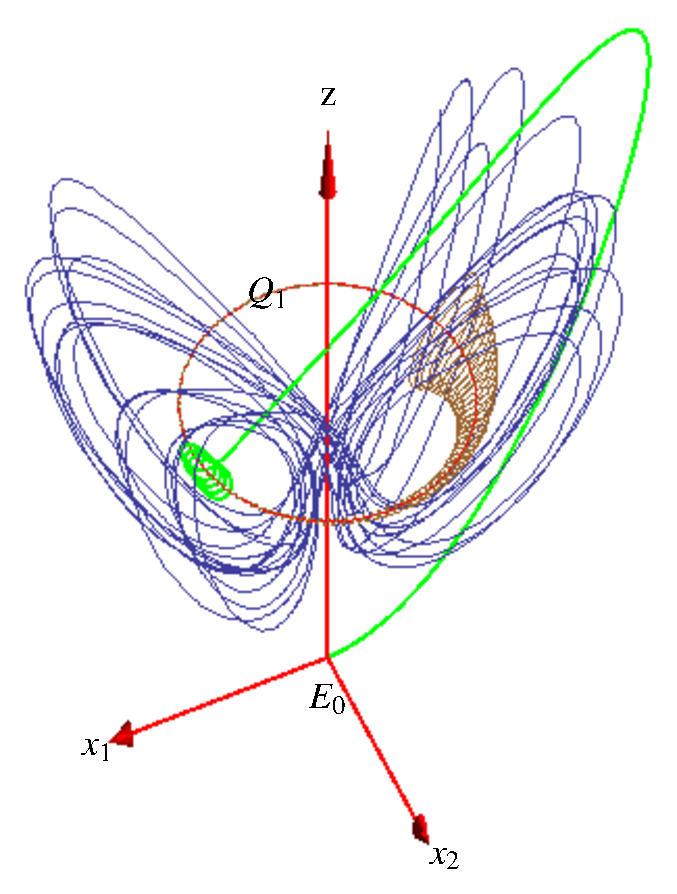
\includegraphics[height=0.25\textheight]{../figs/CLE}
\end{center}
\caption{
\Statesp\ portrait of \cLf. Plotted are \reqv\
\REQV{}{1} (red), its unstable manifold (brown), \eqv\
\EQV{0}, a representative of its unstable manifold (green),
three repeats of the \cycle{01} \rpo\ (magenta), superimposed
over a generic chaotic trajectory (blue).
}
\label{fig:CLE}
\end{figure}
%%%%%%%%%%%%%%%%%%%%%%%%%%%%%%%%%%%%%%%%%%%%%%%%%%%%%%%%%%%%
%
\CLe\ are a dynamical system with a continuous (but no
discrete) symmetry, equivariant under the one-parameter
rotation group $\Un{1}\cong\SOn{2}$ acting by
\beq\label{eq:SO2cle}
	(x,\,y,\,z)\mapsto (
    e^{i\theta}x,\,e^{i\theta}y,\,z)\,,\ \theta\in[0,2\pi]
\,.
\eeq
Alternatively, substituting the Lie algebra generator
    \PC{is the sign standard?}
\beq
 \Lg \,=\,   \left(\barr{ccccc}
    0  & -1 & 0  &  0 & 0  \\
    1  &  0 & 0  &  0 & 0 \\
    0  &  0 & 0  & -1 & 0  \\
    0  &  0 & 1  &  0 & 0 \\
    0  &  0 & 0  &  0 & 0
    \earr\right)
\ee{CLfLieGen}
acting on a 5-dim\-ens\-ion\-al space \refeq{eq:CLeR} into
\refeq{FiniteRot} yields the  $\Rls{5}$ representation of a
finite angle action \refeq{eq:SO2cle} of $\SOn{2}$
\beq
\LieEl(\gSpace) \,=\,  \left(\barr{ccccc}
  \cos \gSpace  & -\sin \gSpace  & 0 & 0 & 0 \\
  \sin \gSpace  &  \cos \gSpace  & 0 & 0 & 0 \\
 0 & 0 &  \cos \gSpace & -\sin \gSpace   & 0 \\
 0 & 0 &  \sin \gSpace &  \cos \gSpace   & 0 \\
 0 & 0 & 0             & 0               & 1
    \earr\right)
\,.
\ee{CLfRots}
We see that the linear action of \SOn{2}\
on the \cLe\ \statesp\ decomposes into the $m=0$ \Group-invariant
subspace ($z$-axis) and  the $m=1$ subspace of multiplicity 2.

The generator $\Lg$ is anti-hermitian,
$\Lg^\dagger = - \Lg$, and the group is compact, its
elements parametrized by $\gSpace \mbox{ mod } 2\pi$. Locally, at
$\ssp \in \pS$, the infinitesimal action of the group is
given by the group tangent field $\groupTan(\ssp) = \Lg \ssp
= (-x_2,x_1,-y_2,y_1,0)$. In other words, the flow induced by
the group action is normal to the radial direction in the
$(x_1,x_2)$ and $(y_1,y_2)$ planes, while the $z$-axis is left
invariant.

That \cLf\ is equivariant
under $\SOn{2}$ rotations \refeq{CLfRots} can be checked
by substituting the Lie algebra generator
\refeq{CLfLieGen} and the \stabmat\ for \cLf\ \refeq{eq:CLeR},
  \beq
\Mvar =
  \left(\barr{ccccc}
    -\sigma    	& 0 		& \sigma & 0    &  0 \\
	0 	& -\sigma       & 0      & \sigma   &  0 \\
	\RerCLor-z  &     -\ImrCLor      & -1     & -e & -x_1 \\
	\ImrCLor     & \RerCLor-z       	& e  	& -1       & -x_2 \\
	y_1     & y_2           & x_1    & x_2      & -b
    \earr\right)
\,,
  \ee{CLeStabMat}
into the equivariance condition \refeq{inftmInv}.
For the parameter values \refeq{eq:CLeR} the flow
is strongly volume contracting,
\beq
\pde_i \pVeloc_i
 = \sum_{i=1}^{5} \Lyap_i(\ssp,t)
= -b -2(\sigma + 1)
= -24 - 2/3
    \,,
\ee{trA-ZM}

Originally, the \cLe\ \refeq{eq:CLe} were introduced by
Gibbon and McGuinness\rf{GibMcCLE82,FowlerCLE82} as a
low-dim\-ens\-ion\-al model of baroclinic instability in the
atmosphere. Ning and Haken\rf{NingHakenCLE90} have shown that
equations isomorphic to \cLe\ also appear as a truncation of
Maxwell-Bloch equations describing a single mode, detuned,
ring laser. They set $e+\ImrCLor=0$ (see \refeq{eq:omegaCLE})
so that \SOn{2}-orbits of detuned \eqva\
exist\rf{FowlerCLE82}. Zeghlache and Mandel\rf{ZeMa85} also
use equations isomorphic to \cLe\ with $e+\ImrCLor=0$ in
their studies of detuned ring lasers. This choice is
`degenerate' in the sense that it leads to non-generic
bifurcations. As existence of \reqva\ in systems with \SOn{2}
symmetry is the generic situation, we follow Bakasov and
Abraham\rf{BakasovAbraham93} who set $\ImrCLor=0$ and $e \neq
0$ in order to describe detuned lasers.

Here, however, we are not interested in the physical
applications of these equations; rather, we study them as a
simple example of a dynamical system with continuous (but no
discrete) symmetries, with a view of testing methods of
reducing the dynamics to a lower-dimensional \reducedsp.
    \PC{looks like one should also read \refref{Abraham95}; they
    report on various return maps}
We investigate
various ways of `quotienting' its \SOn{2} symmetry, and
reducing the dynamics to a 4-dim\-ens\-ion\-al \reducedsp. As
we shall show, the dynamics has a nice {\stretchf}
action, but that is totally masked by the continuous symmetry
drifts. We shall not rest until we attain the simplicity of
\reffig{fig:CLEmfReqb1}, and the bliss of 1-dim\-ens\-ion\-al
return map of \reffig{fig:CLEipRM}.
